% Truc qu'Olivier a tellement insisté
\chapter{Analyse critique}

Prenons maintenant un peu de recul sur ce projet...\\

Au chapitre \ref{chapter:problematique}, nous avons d'abord défini les besoins clés d'une application de partage de \glspl{resinfo} en analysant une série de plateformes web existantes.\\

Après cela, en chapitre \ref{chapter:analyseDesBesoins}, nous nous sommes concentrés sur une analyse plus profonde de notre plateforme en y relatant les fonctionnalités à intégrer avec la méthode \textbf{\textit{MoSCoW}}, les besoins à satisfaire pour que la plateforme puisse être utilisée par le grand public, ainsi que les contraintes qui nous ont été imposées (en incluant celles que nous nous sommes imposées).\\

Dans le chapitre \ref{chapter:solution}, nous avons enfin expliqué notre solution à la problématique du partage de \glspl{resinfo} en détaillant l'architecture de \texttt{SourceCode} aussi bien du côté \gls{frontend} que du \gls{backend}.\\

Dans ce chapitre-ci, nous nous efforçons d'avoir un regard critique sur \texttt{SourceCode}. Par la validation du projet (test avec des utilisateurs externes, test de la qualité du code) et les différentes métriques du projet, nous voulons nous assurer que notre prototype ait un sens et contribue utilement à la problématique des \glspl{resinfo}.

\section{Validation}
\label{section:validation}

\subsection{Validation externe}
\label{section:validationExterne}

Pour valider notre travail, nous avions initialement planifié deux séances de validation afin de récolter les avis d'un panel d'utilisateurs suffisamment large.
Pour cause de COVID-19, il n'a été possible d'organiser qu'une seule, avec sept utilisateurs. Chaque personne se voyait attribuer deux rôles différents (visiteur-utilisateur ou visiteur-administrateur) afin de prendre connaissance des fonctionnalités les plus importantes de \texttt{SourceCode}. Notre évaluation a pu être réalisée grâce à Google Forms (réponses, graphiques) et vous retrouverez l'intégralité de ce sondage dans l'annexe ???.\\

Parmi les participants, six d'entre eux font partie de l'\textit{UCLouvain} de la faculté \textit{EPL}, dont quatre étudiants de master en sciences informatiques et deux doctorants. La septième personne est une professeure en section informatique à la \textit{HELHa} de Mons.\\

Un des premiers objectifs de cette séance fut de faire comprendre le but de la plateforme, son utilité. Cela semblait être acquis par la majorité sauf pour une personne. Il n'est pas exclu de penser que cette dernière était biaisée par la plateforme \textit{INGInious} de l'\textit{UCLouvain}, car elle l'a prise comme point de référence pour juger \texttt{SourceCode}.\\

Les sous-sections suivantes résument les critiques émises sur \texttt{SourceCode}. Certaines remarques suggéraient des améliorations et corrections. Avec le temps qui nous restait, nous avons essayé de les prendre en compte pour rendre l'utilisation de la plateforme un peu plus immersive et plus fonctionnelle. Vous retrouverez alors un "\textbf{(corrigé)}" quand nous avons pu prendre en considération la remarque.

\subsubsection*{Bibliothèque}

\begin{itemize}
    \item Système de recherche intuitif, rapide et riche en filtres.
    \item La barre de recherche n'est pas bien placée, car elle laisse penser que c'est pour lancer une recherche sur tout le domaine du site web. \textbf{(corrigé)}
    \item Dans la création de favoris depuis le panneau, au lieu de cliquer sur OK, appuyer sur enter pour valider le nom du nouveau favori. \textbf{(corrigé)}
    \item Ajouter quelques tags + titre de recherche plutôt que juste le nom du favori dans la partie onglet "favoris". \textbf{(corrigé)}
    \item Recherche : Gestion des fautes de frappe et/ou recherche approximative. (1)
    \item Le texte de la barre de recherche est trop petit, et en bleu trop clair. \textbf{(corrigé)}
    \item Un peu difficile de scroller dans la liste des tags (jusqu'à 3 scrollbars). \textbf{(corrigé)}
\end{itemize}
\bigskip

\begin{enumerate}
    \item La gestion des fautes de frappe ou recherche approximative est une fonctionnalité qui pourrait être très utile pour la bibliothèque (le but étant de faciliter la recherche au maximum).
\end{enumerate}

\subsubsection*{Favoris}

\begin{itemize}
    \item Pas nécessaire d'avoir obligatoirement un tag pour créer un favori. \textbf{(corrigé)}
    \item Quand on crée un favori puis le modifie, difficile de se souvenir de quelle catégorie appartient le tag qu'on a sélectionné précédemment : soit renommer le tag, soit créer un moyen de savoir de quelle catégorie le tag appartient. (1)
\end{itemize}

\bigskip

\begin{enumerate}
    \item Lors de l'édition d'un favori ou d'une \gls{resinfo}, les \glspl{tag} ajoutés sont affichés dans une section du formulaire en mode pêle-mêle (sans les catégories auxquels ils se rapportent). Le seul moyen de vérifier la catégorie à laquelle un \gls{tag} appartient est de naviguer dans le panneau à onglets. Nous discuterons des futures améliorations possibles dans le chapitre ???.
\end{enumerate}


\subsubsection*{Création de \glspl{resinfo}}

\begin{itemize}
    \item Frustrant de ne pas pouvoir créer un bloc de code directement depuis plusieurs lignes sélectionnées. (1)
    \item Ajouter un <tab> pour l'édition du code. \textbf{(corrigé)}
    \item Possibilité d'agrandir la boîte d'édition de texte. (2)
    \item Un peu difficile d'utiliser le panneau des tags (c'est une première) (3)
\end{itemize}

\bigskip
\begin{enumerate}
    \item Actuellement, il faut d'abord créer un bloc de code puis copier-coller le code que l'on veut formater dedans. La \gls{library} d'édition de texte que nous utilisons (Tiptap) ne gère pas nativement ce qui a été soulevé dans la remarque. En revanche, cette même \gls{library} est extensible et autorise la modification/l'ajout de fonctionnalités de manière aisée. Il est donc tout à fait envisageable de corriger le tir dans une prochaine mise à jour de l'application.
    \item Certaines personnes se plaignaient que la boîte d'édition était trop petite (ou trop grande). Dans son état actuel, \texttt{SourceCode} n'est pas responsive, et dans la perspective où elle le serait, ce problème sera certainement réglé pour tout écran.
    \item Comme cela a déjà été soulevé dans la section concernant la bibliothèque, le panneau des \glspl{tag} est un peu lourd à l'utilisation. Il y avait jusqu'à 3 scrollbars pour naviguer dans le panneau, ce qui diminuait considérablement l'accessibilité. Nous avons donc changé ce comportement en faisant en sorte d'afficher une seule scrollbar, avec un accès plus clair à la barre de recherche sous chaque \glspl{tagCat}.
\end{enumerate}

\subsubsection*{Esthétique et ergonomie}

\begin{itemize}
    \item Très chouette.
    \item Le bouton retour dans le header est un peu perturbant, car on ne le remarque pas avant d'avoir vraiment pris en main le site. \textbf{(corrigé)}
    \item Un dark mode (1)
\end{itemize}
\bigskip
\begin{enumerate}
    \item Le dark mode n'est pas une fonctionnalité nécessaire à la plateforme, mais elle pourrait ajouter un plus côté attractivité.
\end{enumerate}

\subsubsection*{Points forts}

\begin{itemize}
    \item Ergonomique et riche en filtres de recherche.
    \item Très complète.
    \item Très utile, s'il y a une grande communauté et qu'il y a beaucoup d'exercices. (1)
    \item La sélection dynamique est top (pour la recherche).
    \item Design, visuel, fluidité.
    \item L'idée de rassembler toutes les ressources informatiques au même endroit semble pertinente et utile.
    \item Le système de tags (utilisé correctement par les utilisateurs) semble flexible et potentiellement très utile.
    \item Visuellement attrayant.
\end{itemize}
\bigskip
\begin{enumerate}
    \item La grande communauté dépendra surtout de la qualité de l'application et de son utilité. Les exercices que nous avons utilisés pour la séance de validation étaient importés à partir de quatre cours hébergés sur la plateforme \textit{INGInious}. Nous pouvons donc aisément fournir plus de contenu rien qu'en important tous les cours stockés sur cette même plateforme avec l'avantage d'un système de \glspl{tag} plus avancé.
\end{enumerate}

\subsubsection*{Points faibles}

\begin{itemize}
    \item S'il y a peu d'exercices, la plateforme aura peu de sens. (1)
    \item S'il y a trop d'exercices, les administrateurs pourraient peut-être demeurer débordés pour la modération. (2)
    \item L'application est très complète, mais le souci vient justement de cela : la courbe d'apprentissage est assez pentue, mais après cela, l'outil deviendrait très puissant (difficulté pour les professeurs un peu moins "tech savvy"). (3)
\end{itemize}

\bigskip
\begin{enumerate}
    \item \texttt{SourceCode} pourra très rapidement posséder une riche bibliothèque de \glspl{resinfo} rien qu'avec les exercices stockés sur la plateforme \textit{INGInious}. Avec la promotion de la plateforme auprès d'autres institutions scolaires, \texttt{SourceCode} pourrait alors prétendre à une popularité certaine dans le monde des ressources partagées. Il s'agit alors de savoir vendre son produit avec les bons arguments...
    \item Nous n'avions pas pensé à cela pour le prototype. Nous voulions d'abord créer un système cohérent et fonctionnel au niveau de la gestion des \glspl{resinfo} et \glspl{tag}. Les différents statuts attribuables à ces mêmes \glspl{resinfo} et \glspl{tag} jouent déjà un rôle majeur dans la gestion (ex: trier les \glspl{resinfo} non valides ou en attente de validation ...). En termes d'améliorations, nous pourrions automatiser le processus de validation afin que les administrateurs ne soient pas débordés (voir chapitre ???).
    \item C'est un point intéressant pour nous. \texttt{SourceCode} est une application qui tente de faciliter le plus possible la recherche et la gestion de \glspl{resinfo} (système de filtres, historique, favoris ...). Malheureusement, ajouter une pléthore de fonctionnalités peut aussi devenir une barrière à l'utilisation, car l'utilisateur doit d'abord apprendre à les maîtriser. Une des premières solutions que nous avons mises en place était la création d'une section tutoriel sur la plateforme, mais cela n'est qu'une solution de contournement. Il faut que la plateforme puisse évoluer en termes d'ergonomie pour rendre l'interface plus accessible aux utilisateurs.
\end{enumerate}

\subsubsection*{Que pouvons-nous faire pour améliorer l'application ?}

\begin{itemize}
    \item Il s'agit d'un produit bien abouti ! Vous êtes à un stade où ça sera les utilisateurs de la plateforme qui vous feront des feedbacks sur ce qui serait bien à ajouter/améliorer.
    \item Clarifier l'interface. L'UI représente cependant beaucoup de travail. Vous avez priorisé les bonnes choses.
    \item Améliorer l'agencement des menus. (1)
    \item Une fonction mot de passe oublié pour les utilisateurs. (2)
\end{itemize}
\bigskip
\begin{enumerate}
    \item Dans les retours d'utilisation, les testeurs étaient perturbés avec le menu principal et le panneau latéral. La confusion venait du fait que le menu principal comportait des chevrons, ce qui laissait penser à une structure à plusieurs niveaux (listes). Le panneau de filtres contenait aussi ces mêmes chevrons, alors nous avons supprimé ces derniers sur le menu principal pour enlever cette confusion.
    \item C'est une fonctionnalité importante pour ce genre d'application, mais nous n'avons pas pris le temps de l'intégrer. Nous l'ajoutons dans le chapitre ???
\end{enumerate}

\subsubsection*{Que manquerait-il pour que cette plateforme ne soit plus un prototype en termes de fonctionnalités ?}

\begin{itemize}
    \item Je ne vous rejoins pas sur l'idée que Source Code en est au stade de "prototype". Ça ressemble bien plus à un produit fini, en une première version, qui peut être concernée par d'éventuelles mises à jour par la suite.
    \item Pas grand-chose, et beaucoup à la fois. Il s'agit du lent travail de lisser les bugs et les surprises que peuvent rencontrer les utilisateurs.
    \item Peut-être la complétion automatique dans la barre de recherche
    \item Pour moi c'est plus qu'un prototype au stade où elle en est. S'il fallait vraiment une fonctionnalité en plus, ça serait de pouvoir ajouter ses solutions sur la plateforme. (1)
    \item Une manière d'interagir entre les étudiants et les "créateurs d'exercices" ? Histoire de pouvoir au moins poser des questions et ne pas être aussi détachés. (2)
\end{itemize}
\bigskip
\begin{enumerate}
    \item \texttt{SourceCode} n'est pas prévu pour résoudre des exercices depuis la plateforme. À ce stade-ci, on peut la considérer comme un référenceur de \glspl{resinfo} qui faciliterait la recherche de ressources particulière avec un système de recherche complet. Dans une perspective future, \texttt{SourceCode} pourrait avoir son propre correcteur d'exercices si la ressource nécessite une résolution. Dans ce cas, cela profiterait aux étudiants pour s'évaluer.
    \item Certaines plateformes comme Hackerrank ou Coderbyte ont prévu une section forum pour chaque exercice/challenge. C'est une fonctionnalité intéressante, mais elle va de pair avec le point précédent.
\end{enumerate}

\subsubsection*{Pensez-vous que cette application ait un réel impact dans le monde des ressources partagées ?}

\begin{itemize}
    \item Oui (de la part de la majorité)
    \item Il faudrait juste voir comment gérer l'accès entre votre plateforme et celles qui permettent la correction des exercices (Inginious). Par exemple un moyen de linker votre plateforme avec les autres, pour qu'en un clic on arrive directement sur l'exercice inginious en étant déjà connecté dessus.
    \item Sans être intégrée à une plateforme automatisée de correction de code, et sans une gestion de parcours et de lien entre les exercices, sans doute pas beaucoup. Elle sera limitée à une utilisation par les enseignants pour créer leurs propres cours.
\end{itemize}
\bigskip
\begin{enumerate}
    \item 
    \item La plateforme est d'abord créée pour l'équipe pédagogique, prônant le partage de \glspl{resinfo} dans une bibliothèque triée par \glspl{tag}. Une prochaine étape serait alors d'intégrer un système de correction d'exercices directement depuis la plateforme. Nous n'avions pas eu le temps d'intégrer une telle fonctionnalité, mais cela pourrait définitivement être utile aux étudiants.
\end{enumerate}

\subsubsection*{Utiliseriez-vous cette plateforme ? Quelle serait votre activité principale ?}

\begin{itemize}
    \item Je pense que pour des professeurs, cela peut être très utile pour trouver et donner des exercices à des étudiants (ou d'avoir des idées).
    \item Trouver des idées d'exercices pour compléter mes cours.
    \item Je pense que ça s'appliquerait surtout au domaine éducatif.
    \item Oui, en tant que professeur/enseignant, pourvu que les solutions soient mises à dispositions. (1)
\end{itemize}
\bigskip
\begin{enumerate}
    \item 
\end{enumerate}

\subsubsection*{Conclusion}

Cette séance de validation a globalement été positive et instructive. Le message d'une plateforme de partage de \glspl{resinfo} à destination d'une équipe pédagogique semble être acquis par la majorité. 
Nous avons appris que la plateforme dispose d'un design et d'une ergonomie satisfaisants. Il faut néanmoins y apporter quelques mises à jour pour rendre le projet mature, notamment au niveau de l'ergonomie.
Certaines des fonctionnalités mentionnées dans les critiques ont pu être intégrées à \texttt{SourceCode} pour l'améliorer le plus possible. Pour celles qui n'ont pas été ajoutées, nous les avons référencées dans le chapitre ???.

\subsection{Code coverage}
\label{section:codeCoverage}

Le \gls{backend} a aussi eu sa forme de validation avec un ensemble de tests pour s'assurer que l'\gls{api} fait bien ce qu'on attend d'elle.\\

Nous avons principalement utilisé le \textit{branch coverage}, dont nous allons vous expliquer son fonctionnement avec un exemple.\\

\begin{figure}[H]
    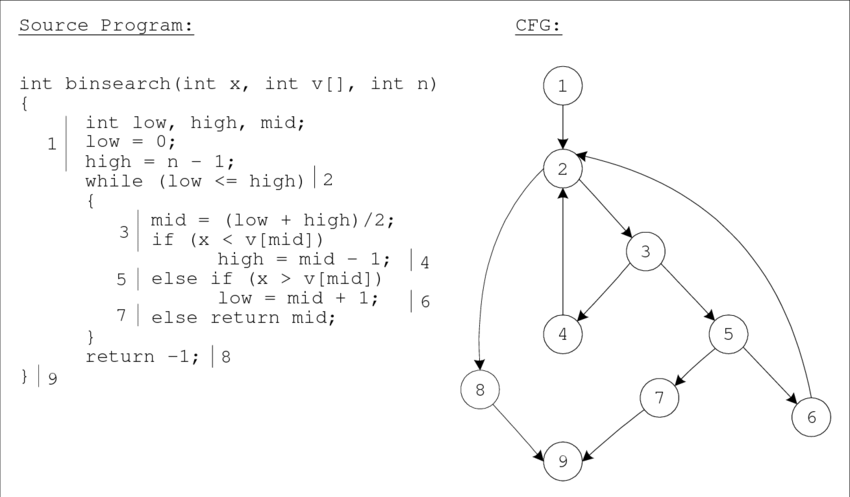
\includegraphics[width=\textwidth,height=0.3\textheight,keepaspectratio]{images/analyseCritique/CFG.png}
    \centering
    \caption{Exemple d'un CFG pour le branch coverage}
\end{figure}

Sur cette image illustrant la méthode \texttt{binsearch} (recherche binaire), nous pouvons découper en plusieurs parties le code afin de dessiner le schéma présenté sur la droite. Ce dernier désigne un graphe de flot de contrôle (GFC) représentant tous les chemins qui peuvent être suivis par un programme lors de son exécution.\\

Pour le \textit{branch coverage}, on dit que chaque branche doit être exécutée au moins une fois. Dans le cas du GFC, cela se traduit par le passage sur chaque arête au moins une fois.\\

Mesure : $ C_{branche} =  \frac{\# \; branches \; exécutées}{\# \; branches}  $\\

Avec 48 tests, nous avons pu atteindre une couverture maximale (100\%), car chaque méthode a été testée extensivement avec le \textit{branch coverage}.\\

Vous pouvez d'ailleurs consulter les résultats depuis \url{https://codecov.io/gh/SourceCodeOER/sourcecode_api/list/master/}.



\section{Métriques}

Cette section traduit notre implication sur ce projet. Pour ce faire, nous avons repris des statistiques des répertoires GitHub du \gls{frontend} et de l'\gls{api}. La notion la plus intéressante à prendre en compte sera le graphe d'activité pour les deux répertoires, car nous avons tenté de respecter le planning imposé (voir \ref{pic:ganttChart}).

\subsection{Statistiques}

\begin{itemize}
    \item Nombre de lignes de code (frontend + backend) : 21685 + 10158 = 31843
    \begin{itemize}
        \item Le nombre de lignes de code a été calculé en retirant tous les fichiers générés automatiquement par un script (ex : npm install qui va créer un fichier \textit{package-lock.json}).
    \end{itemize}
    \item Nombre de pull requests résolues (frontend + backend) : 49 + 79 = 128
    \begin{itemize}
        \item Nous avons beaucoup utilisé les pull requests avec GitHub car nous voulions garder une trace des mises à jour importantes effectuées. Elles ont aussi été extrêmement utiles avec l'intégration continue de \textit{Docker} qui nous permettait de rapidement tester l'application avec l'une d'elles.
    \end{itemize}
\end{itemize}

\subsection{Graphe d'activité}

\texttt{SourceCode} a connu un développement plus ou moins constant durant l'année académique 2019-2020. Étant donné que le \gls{frontend} et le \gls{backend} sont intimement liés, vous pourrez constater sur le graphe \ref{figure:frontendActivity} et \ref{figure:backendActivity} que la forte activité de l'un compense l'activité au ralenti de l'autre répertoire.

\begin{figure}[H]
    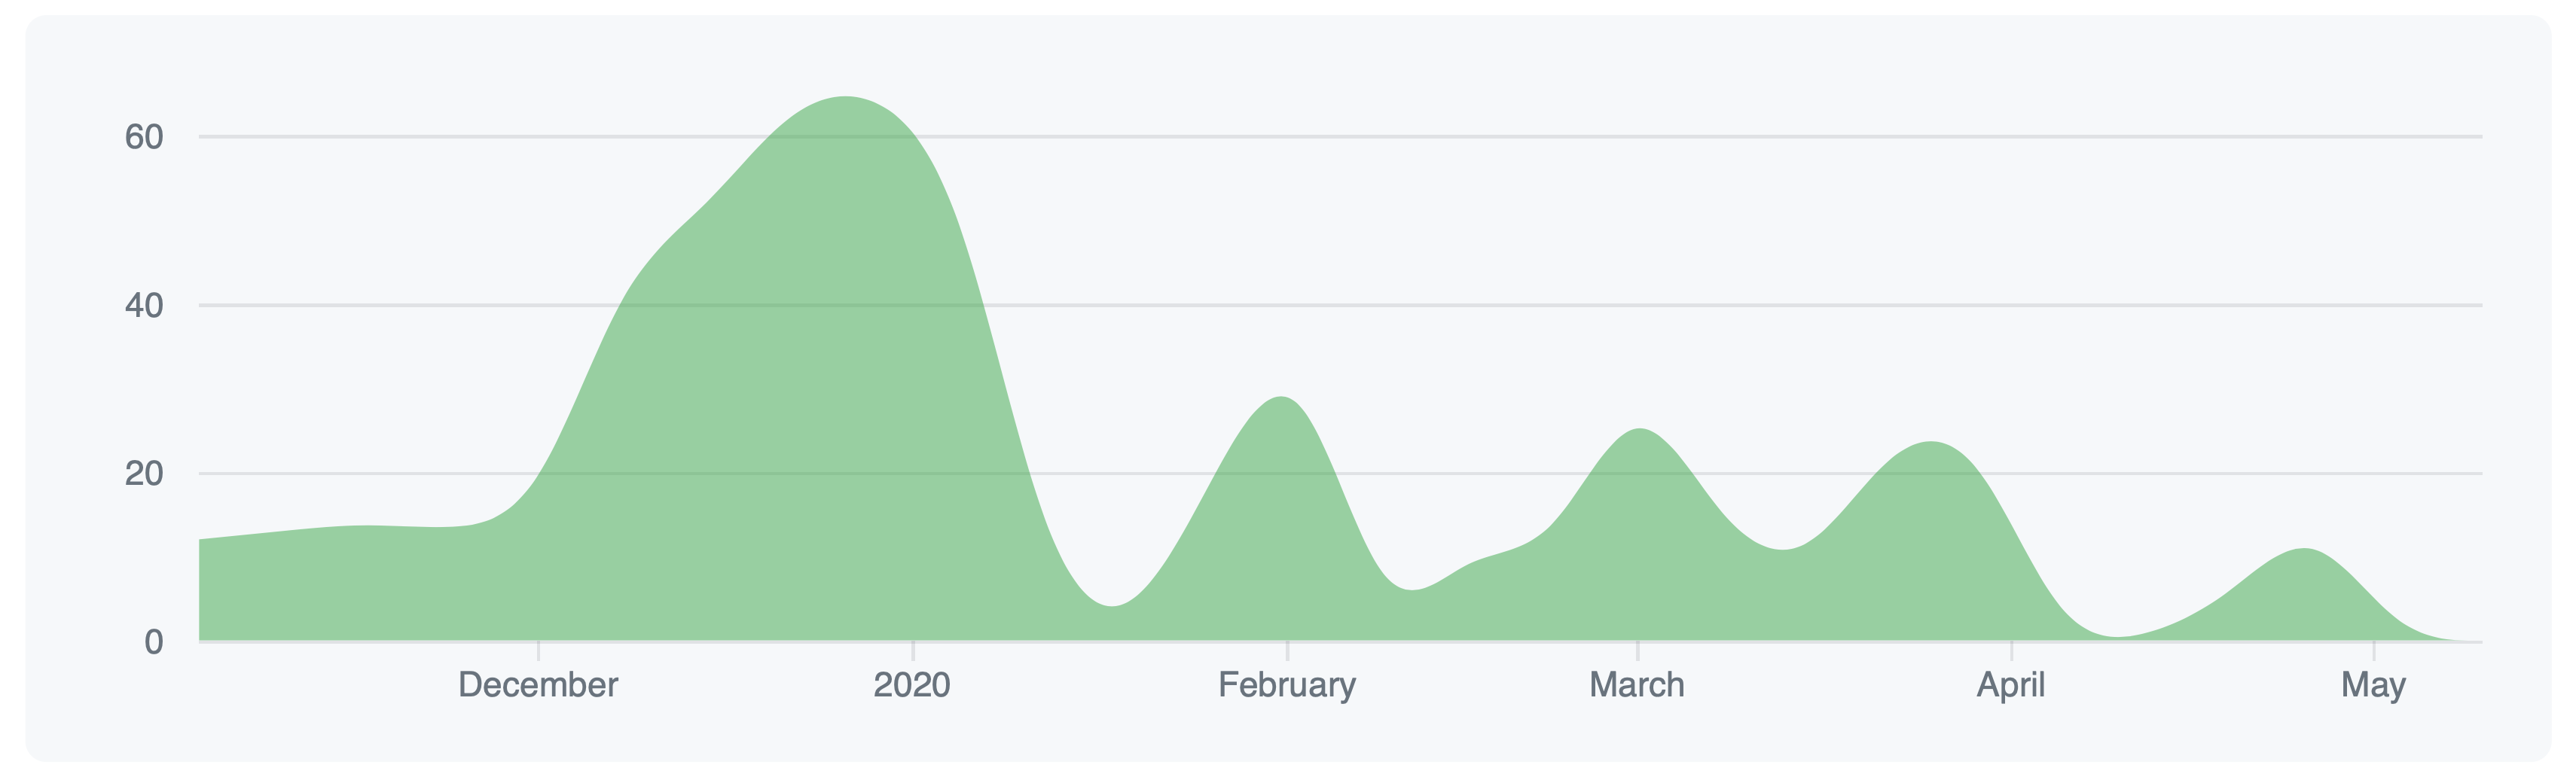
\includegraphics[width=\textwidth,height=0.3\textheight,keepaspectratio]{images/analyseCritique/graph_frontend.png}
    \centering
    \caption{GitHub : graphe d'activité (frontend)}
    \label{figure:frontendActivity}
\end{figure}

Les fonctionnalités les plus importantes comme la recherche dans la bibliothèque, la consultation d'une \gls{fiche} et la gestion des \glspl{resinfo} ont été intégrées durant la période d'octobre à janvier, après quoi nous avons amélioré l'expérience d'utilisation de l'application en appliquant quelques mises à jour et corrections de bugs jusqu'au mois de mai.\\

\begin{figure}[H]
    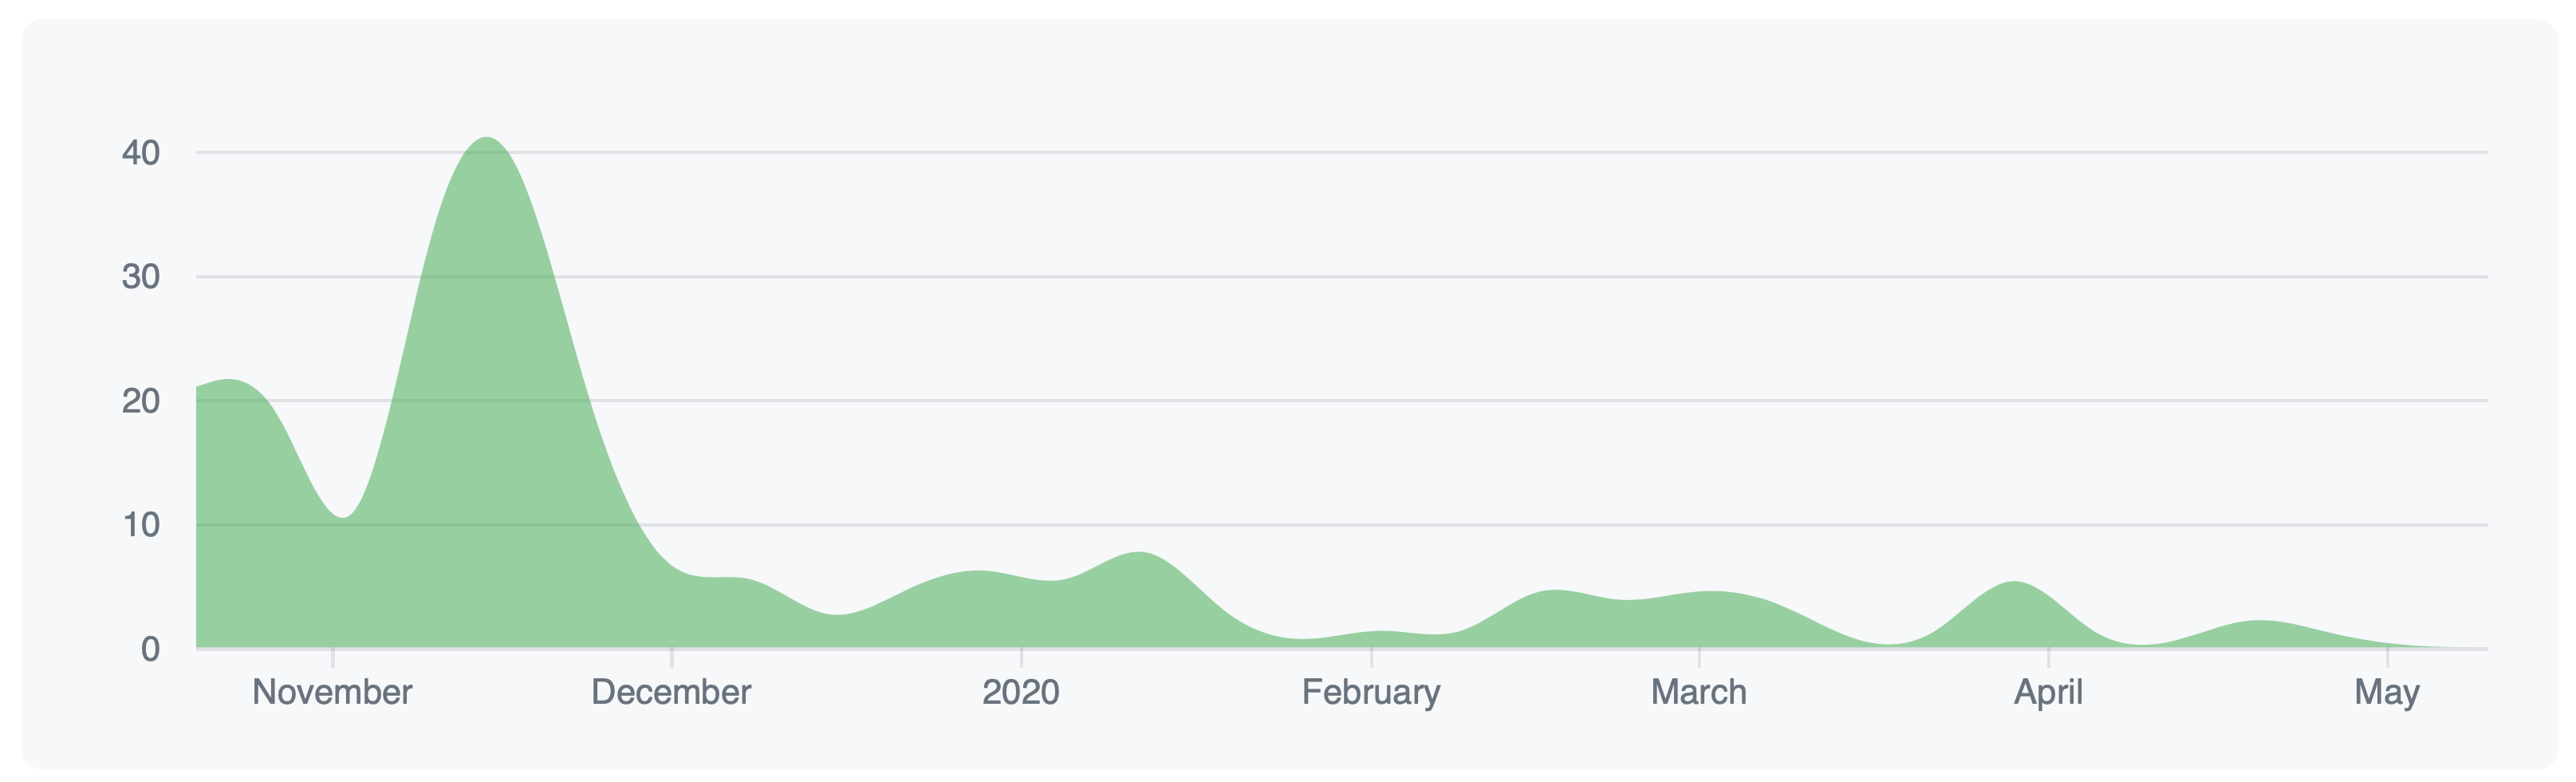
\includegraphics[width=\textwidth,height=0.3\textheight,keepaspectratio]{images/analyseCritique/graph_backend.png}
    \centering
    \caption{GitHub : graphe d'activité (backend)}
    \label{figure:backendActivity}
\end{figure}


Globalement, nous avons respecté le planning \ref{pic:ganttChart} que nous nous sommes imposés. Nous avons cependant effectué une dernière mise à jour prenant en compte un maximum des remarques relatées en section \ref{section:validationExterne}, car nous voulions prouver que \texttt{SourceCode} est capable de s'adapter aux besoins des utilisateurs.

\subsection{Conclusion}

Ce chapitre était agréable à rédiger car nous avons pu constater si \texttt{SourceCode} est un projet qui tient la route à son stade de développement.\\

La séance de validation nous a été extrêmement bénéfique, car les remarques étaient constructives. Cela nous conforte dans l'idée que notre plateforme a des chances de devenir mature et utilisable par une communauté. Quoi qu'il en soit, notre projet est \textit{Open Source} et pourra donc toujours évoluer avec sa communauté. C'est d'ailleurs notre plus grand souhait pour cette plateforme.\\

Au niveau du planning, il semble que nous ayons respecté ce qui était initialement mis en place au vu de nos graphes d'activité. Nous avons tenté d'être constants tout au long du projet, car ce dernier demande beaucoup d'investissement en matière de recherche et de développement. Il semblerait que cela ait porté ses fruits.